\RequirePackage{luatex85}
\documentclass{standalone}

\usepackage{amsmath}

\usepackage{fontspec, unicode-math}
\setsansfont[Scale=MatchLowercase]{TeX Gyre Heros}
\setmathfont{TeX Gyre Termes Math}

\usepackage{tikz}
\usetikzlibrary{shapes}
\usepackage{pgfplots}
\pgfplotsset{compat=1.14}

\tikzset{
  every picture/.style={font={\sffamily\normalsize}, >=stealth},
  every pin edge/.style={black}}

\begin{document}

  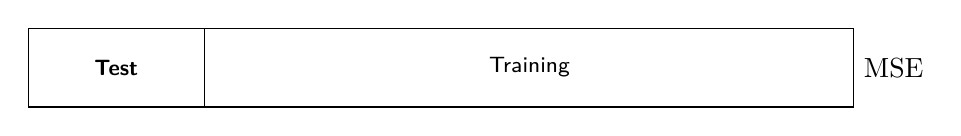
\begin{tikzpicture}[
    kFold/.style={
      draw, font=\sffamily\footnotesize,
      align=center,
      rectangle split,
      rectangle split horizontal,
      minimum height=1cm},
    test/.style={text width=2cm}]

    \node[kFold, rectangle split parts=2] at (0, 3) [
           label=0:$\mathrm{MSE}$]
    {
      \nodepart[text width=8cm]{two}Training
      \nodepart[test]{one}{\sffamily\bfseries Test}
    };
  \end{tikzpicture}

\end{document}
